In this section the basic concepts of process mining, long short-term memory networks, text mining as well as necessary formal definitions and notations are defined.


%\begin{figure}
	%\centering
	%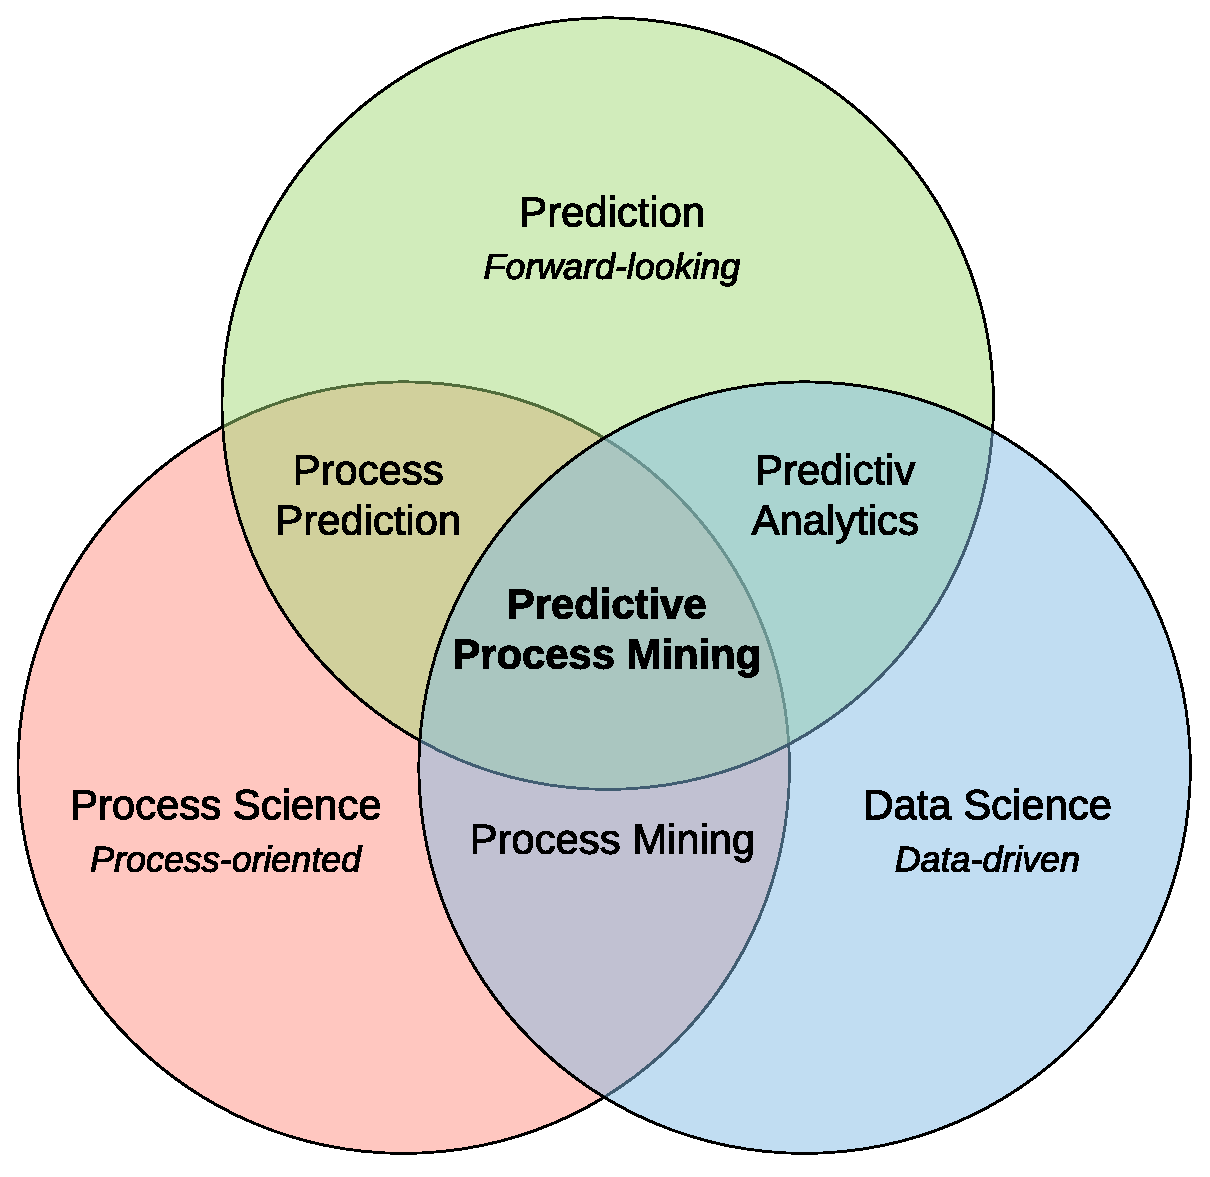
\includegraphics[width=0.5\textwidth]{figures/predictive-process-mining}
	%\caption{Predictive Process Mining combines the concepts of process science, data %science and prediction}
%\end{figure}


\section{Processes and Process Mining}

A \textit{business process} is a collection of activities that are performed in a specific order to archive a goal \cite{DBLP:conf/bpm/AalstAM11}.
A single execution of a process is a \textit{case} or \textit{process instance}, which is identified by a case ID.
Each performed activity belongs to specific case and is completed at a certain time.
A case can be e.g. a patient in a hospital, a customer of a company or an order and is usually identified by an ID, while 
the time is specified by a timestamp.
The trinity of case, activity and timestamp is called event.
An event can have more attributes like describing the resource, costs or transactional information of the event.

\begin{table}[]
	\begin{tabularx}{\textwidth}{@{}lllllll@{}}
		\toprule
		\textbf{ID} & \textbf{Activity}          & \textbf{Timestamp} & \textbf{Resource} & \textbf{Cost} & \textbf{Comment}                                                                                                & \textbf{...} \\ \midrule
		0                & Register patient           & 01.02.2020:14.12   & SYSTEM            & 0             & -                                                                                                               & ...          \\
		& Consultation               & 01.02.2020:14.34   & John Brown, MD    & 24.32         & \begin{tabular}[c]{@{}l@{}}The patient reports persistent\\ nausea.\end{tabular}                                & ...          \\
		& Blood test                 & 01.02.2020:15.12   & Kim Smith         & 14.23         & Tests: Complete blood count                                                                                     & ...          \\
		& Evaluate test result       & 01.02.2020:16.35   & John Brown, MD    & 38.67         & \begin{tabular}[c]{@{}l@{}}No abnormalities in the complete\\ blood count.\end{tabular}                         & ...          \\
		& Release patient            & 01.02.2020:17.24   & SYSTEM            & 0             & -                                                                                                               & ...          \\
		&                            &                    &                   &               &                                                                                                                 &              \\
		1                & Register patient           & 02.02.2020:08.20   & SYSTEM            & 0             & -                                                                                                               & ...          \\
		& Consultation               & 02.02.2020:14.12   & Jana Simpson, MD  & 24.32         & \begin{tabular}[c]{@{}l@{}}Noticeable tachycardia. No chronic pre-existing conditions\\ are known.\end{tabular} & ...          \\
		& MRI & 02.02.2020:14.12   & Sara Taylor, MD   & 352.87        & -                                                                                                               & ...          \\
		& Release patient            & 02.02.2020:14.12   & SYSTEM            & 0             & -                                                                                                               & ...          \\
		&                            &                    &                   &               &                                                                                                                 &              \\
		2                & Register patient           & 02.02.2020:09.08   & SYSTEM            & 0             & -                                                                                                               & ...          \\
		& Consultation               & 02.02.2020:09.14   & Jana Simpson, MD  & 24.32         & \begin{tabular}[c]{@{}l@{}}The patient has severe leg injuries\\ due to a motorcycle accident.\end{tabular}     & ...          \\
		& Patient hospitalized       & 02.02.2020:09.20   & Mike Johnson      & 130.37        & -                                                                                                               & ...          \\
		...              & ...                        & ...                & ...               & ...           & ...                                                                                                             & ...          \\ \bottomrule
	\end{tabularx}
	\caption{Artifical event log of patient treatment in a hospital}
	\label{tab:event-log}
\end{table}

If the execution of a business process is logged by an information system, the resulting event data is called \textit{event log}.
Depending on the format of the event log, it can also contain additional data on case level.
Typical formats for event logs, which are not part of an database, are comma-separated values (CSV) and eXtensible Event Stream (XES) \cite{DBLP:conf/caise/VerbeekBDA10a}.
A table-based representation of an artificial event log can be seen in Table \ref{tab:event-log}.

Process mining is the discipline that covers all approaches aiming to generate value out of event data.
As an umbrella term, Process Mining includes or utilizes concepts of Business Process Management, Data Mining, Business Process Intelligence, Big Data, Workflow Management, Business Activity Monitoring \cite{DBLP:books/sp/Aalst16} as well as Machine Learning \cite{DBLP:conf/bpm/VeitGMHT17}.

Process mining can be divided into a set of subdisciplines mainly process discovery, conformance checking, process enhancement and process analytics \cite{DBLP:conf/caise/EckLLA15}.
Process discovery aims to generate process models out of event data in order to understand a process and enable further analysis.
Conformance checking is about comparing the intended and observed behavior of a process. 
On top of these diagnostic approaches, process enhancement deals with the improvement of processes.

Driven by the fast and ongoing development of quantitative prediction methods in data science and machine learning, prediction-based methods have been applied to event data leading to process prediction, a major subfield in process analytics.
Forecasting the future of a running process instance is one of the main goals in process prediction and also the main topic of this thesis.


\section{Basic notations, Sequences and Functions}

The set $\mathbb{N}$ denotes the set of all natural numbers $\{1, 2, 3, \dots\}$, while $\mathbb{N}_0 = \mathbb{N} \cup \{0\}$ denotes the set of natural numbers including 0.
Given a set $A$, $A^n$ describes the set of all sequences $\langle a_1, a_2, \dots, a_n\rangle$ over $A$ of length $n$ with $a_i \in A$, $1 \leq i \leq n$.
The set $A^0$ is defined as $\{\langle \rangle\}$, where $\langle \rangle$ is the empty sequence of length $0$.
The set of all possible sequences over $A$ is given with $A^* = \bigcup\limits_{i\in \mathbb{N}_0} A^i$.

Sequences $\sigma_1$, $\sigma_2$ can be concatenated to $\sigma_1 \cdot \sigma_2$.
Moreover, the $i$th element of a sequence $\sigma = \langle a_1, a_2, \dots, a_n\rangle$ is accessed by $\sigma(i)= a_i$ for $1 \leq i \leq n$.
To derive a subsequence of $\sigma$ we write $\sigma(i,j)=\langle a_i, a_{i+1} \dots, a_j\rangle$ with $1 \leq i < j \leq n$.
The length of a sequence is denoted by $|\sigma|$. If a sequence $\sigma$ contains an element $a_i$, we also write $a_i \in \sigma$.

A function $f \in A \rightarrow B$ can be lifted to sequences $\sigma$ over $A$ element-wise, precisely:

	\[
	f(\sigma) =
	\begin{cases}
	\langle \rangle & \text{if $\sigma = \langle \rangle$} \\
	\langle f(a_1), f(a_2), \dots, f(a_n)\rangle & \text{else} 
	\end{cases}
	\]


\section{Events, Traces, Event logs}

\begin{definition}
An  \textit{event} is defined by tuple $e = (a,c,t,d_1,\dots, d_m) \in \mathcal{C} \times \mathcal{A}  \times \mathcal{T} \times \mathcal{D}_1 \times \dots \times \mathcal{D}_m =  \mathcal{E}$ where  $c \in \mathcal{C} $ is the case id, $a \in \mathcal{A}$ is the executed activity and $t \in \mathcal{T}$ is the timestamp of the event.
Furthermore, each event contains a fixed number $m \in \mathbb{N}_0$ of additional attributes $d_1 \dots d_m$ in their corresponding domains $\mathcal{D}_1, \dots , \mathcal{D}_m$.
In case that no additional attribute data is given ($m = 0$) the event space $\mathcal{E}$ (set of all possible events) is reduced to $\mathcal{C} \times \mathcal{A}  \times \mathcal{T}$.
\end{definition}

Each attribute $d \in \mathcal{D}$ of an event (including activity, timestamp and case ID) can be accessed by a projection function $\pi_D \in \mathcal{E} \rightarrow \mathcal{D}$.
For example, the activity $a$ of an event $e$ is retrieved by $\pi_\mathcal{A}(e) = a$.

Throughout this thesis,  $\mathcal{C} = \mathbb{N}_0$, $|\mathcal{A}| < \infty$ and $ \mathcal{T} = \mathbb{R}$ is assumed, where $t \in \mathcal{T}$ is given in Unix time, precisely the number of seconds since 00:00:00 UTC on 1 January 1970 minus the applied leap seconds.
Each additional attribute is assumed to be numerical, categorical or textual, i.e. $\mathcal{D}_i = \mathbb{R}$, $|\mathcal{D}_i| < \infty$ or $\mathcal{D}_i = \Sigma^\ast$  for $1 \leq i \leq m$ and some fixed Alphabet $\Sigma$.

\begin{definition}
	A \textit{trace} is a finite and non-empty sequence of events $\sigma = \langle e_1, e_2, \dots\rangle \in  \mathcal{E}^\ast$ with increasing timestamps, i.e. $\pi_\mathcal{T} (e_i) < \pi_\mathcal{T} (e_j) $ for $1 \leq i < j \leq |\sigma|$.
\end{definition}


By lifting the projection functions to sequences a trace can be transformed into a sequence of attributes by applying the projection function to the trace.
For example, $\pi_\mathcal{A}(\sigma)$ gives the sequence of the activities of the events in $\sigma$.

\begin{definition}
	An \textit{event log} $\eventlog = \{ \sigma_1, \sigma _2, \dots, \sigma_k \}$ is a set of traces, where each event of a trace is unique in the log and all events of a trace share a case IDs, which is unique per trace.
\end{definition}

\section{Text mining}

Text mining describes all techniques to generate value out of unstructured or semi-structured textual data.
It combines concepts of natural language processing, machine learning and data mining \cite{DBLP:journals/coling/Mihalcea08}.
The base object in text mining is a \textit{document} containing textual data.
The text can be completed unstructured, i.e. it does not conform to a pre-defined data model, or semi-structured, like in an e-mail, where text information is assigned to sender, subject, message etc.
A collection of documents is called \textit{text corpus}, which forms the basis for many text mining techniques.

In order to derive a mathematical representation of the text data that can be interpreted by a computer, a text model has to be build using the text corpus.
Popular text models are Bag-of-words, Bag-of-n-gram, Paragraph vector (a.k.a. Doc2Vec) \cite{DBLP:conf/icml/LeM14} and Latent Dirichlet Allocation \cite{DBLP:journals/jmlr/BleiNJ03}.
Most models require a text preprocessing step, where the text is cleaned from linguistic variation as well as meaningless words and symbols.


\section{Long short-term memory networks}

Long short-term memory (LSMT) is an advanced recurrent neural network architecture for sequential data originally presented by \citeauthor{DBLP:journals/neco/HochreiterS97} in \citeyear{DBLP:journals/neco/HochreiterS97}  \cite{DBLP:journals/neco/HochreiterS97}.
This approach addresses the well-known vanishing and exploding gradient problem \cite{DBLP:conf/icml/PascanuMB13}  of traditional recurrent neural networks by introducing more complex LSTM cells as hidden units.
The proposed architecture has been improved several times \cite{DBLP:journals/neco/GersSC00} \cite {DBLP:journals/tnn/GreffSKSS17} and considered as one of the most successful recurrent neural network models.
Although LSTM networks have been available for a long time, the breakthrough of this technology is dated around 2016 after many success stories of LSTM in combination with large data sets and GPU hardware have been reported for sequence to sequence tasks like text translation \cite{DBLP:journals/corr/WuSCLNMKCGMKSJL16}.

Gated recurrent units (GRU) \cite{DBLP:conf/emnlp/ChoMGBBSB14} are the competing gating mechanism by \citeauthor{DBLP:conf/emnlp/ChoMGBBSB14} that have fewer parameters and perform similar to LSTM.
However, more recent studies show, that LSTM outperforms GRU consistently in neural machine translation tasks \cite{DBLP:journals/corr/BritzGLL17}.

A simple feedforward neural networks consists of an input layer, arbitrarily many hidden layers and an output layer, where each layer consists of neurons that compute and output the weighted sum of the cells of the previous layer that has been passed to an activation function \cite{DBLP:journals/nn/Schmidhuber15}.
These networks can learn and compute complex functions in supervised learning settings, where input and output pattern are provided.
The network computes a loss function for each training pattern and adjusts its weights with gradient descents using a back-propagation algorithm in order to minimize the loss function \cite{rumelhart1986learning}.

Recurrent neural networks extend traditional feed forward networks with backfeeding connections between hidden layers.
This enables the network to keep a state across inputs and allows the neural network to process arbitrarily long sequences of input data while learning temporal dependencies.

In LTSM networks the layers are replaced by more complex LSTM modules, where each module contains four different sublayers.
The module uses as input the state $C_{t-1}$ and the hidden output $h_{t-1}$ of the module in the previous time step as well as the output of the previous layer $x_t$ to compute a new cell state $C_{t}$ and a (hidden) output $h_{t}$.

\begin{figure}[htbp!]
	\centering
	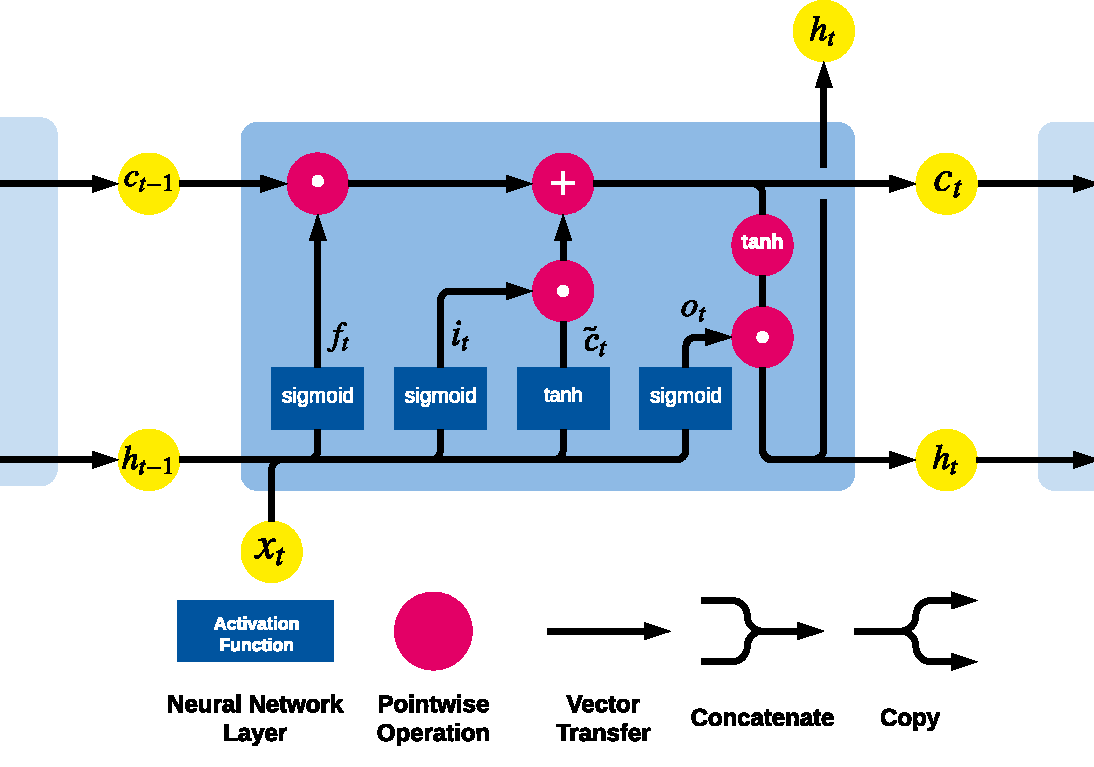
\includegraphics[width=0.8\textwidth]{figures/lstm-module}
	\caption{An LSTM module with four sublayers that manipulate the cell state and compute the module's output. Graphic is adapted from \cite{lstm-blog}}.
	\label{fig:lstm-module}
\end{figure}

The input vector $x_t$ is concatenated with the previous hidden output $h_{t-1}$ and fed to four neural network layers, which are designed to decide what part of the cell state will remain (forget gate $f_t$), how it is updated (update gate $i_t$ and 	$\bar{C}_t$) and what the output of the layer will be (output gate $o_t$ leading to $h_t$).
The sublayer have pointwise $\text{sigmoid}(x) = \frac{1}{1+\mathrm{e}^{-x}}$ or $\tanh(x) = \frac{\mathrm{e}^{x} - \mathrm{e}^{-x}}{\mathrm{e}^{x} + \mathrm{e}^{-x}}$ activation functions, leading to the following equations:

\begin{equation}\label{key}
	f_t = \text{sigmoid}(W_f \cdot [h_{t-1}, x_t] + b_f)
\end{equation}

\begin{equation}\label{key}
	i_t =  \text{sigmoid} (W_i \cdot [h_{t-1}, x_t] + b_i)
\end{equation}

\begin{equation}\label{key}
	\bar{C}_t = \tanh (W_C \cdot [h_{t-1}, x_t] + b_C)
\end{equation}

\begin{equation}\label{key}
	o_t =  \text{sigmoid} (W_o \cdot [h_{t-1}, x_t] + b_o)
\end{equation}

$W_f$, $W_i$, $W_C$ and $W_o$ are the sublayer's learned weights and $b_f$, $b_i$, $b_C$ and $b_o$ are the corresponding biases.

The new cell state $C_t$ is then a combination of the old cell state $C_{t-1}$ and the result of the update gate $\bar{C}_t$, where the layer computations $f_t$ and $i_t$ determine the proportions by a pointwise multiplication ($\odot$) with the cell states.

\begin{equation}\label{key}
	C_t = f_t \odot C_{t-1} + i_t \odot \bar{C}_t
\end{equation}

The result of the output gate $o_t$ is point-wise multiplied with the tanh-activated new cell state to calculate the hidden output $h_t$ of the module.

\begin{equation}\label{key}
	h_t = o_t \odot \tanh(C_t )
\end{equation}

LSTM networks are able to backpropagate a more stable error with this gating mechanism, such that these networks are much more capable of learning complex functions for sequences compared to standard recurrent neural networks.